% Marfa lights model paper -- target: American Journal of Physics (regular article).
% Build:  latexmk -pdf marfa_ajp.tex      (REVTeX 4.2; figures are read from ../figures/)
% For anonymous review set \anonymoustrue: author, affiliation, repository and photographer are withheld.
\documentclass[aip,jap,amsmath,amssymb,reprint,floatfix]{revtex4-2}
\usepackage{graphicx}
\usepackage{dcolumn}
\usepackage{bm}
\usepackage{url}
\usepackage[hidelinks]{hyperref}
\graphicspath{{../figures/}}

\newif\ifanonymous
\anonymousfalse
\ifdefined\anonbuild\anonymoustrue\fi
\newcommand{\repo}{\ifanonymous[repository withheld for review]\else\url{https://github.com/zacharyslate/marfa-lights-investigation}\fi}
\newcommand{\kc}{k_{\mathrm{crit}}}

\begin{document}

\title{Where headlights can hide: line of sight, refraction, and photometry of distant car lights at Marfa, Texas}

\ifanonymous
\author{[Author withheld for review]}
\else
\author{Zach Warren}
\email{zachary.s.warren.85@gmail.com}
\affiliation{[Affiliation to be added]}
\fi

\date{\today}

\begin{abstract}
The ``Marfa lights'' are lights seen at night from a roadside viewing area in West Texas, looking toward the Chinati Mountains. Spectroscopy has shown that many of them are vehicle headlamps, yet observers continue to report lights that appear and vanish, flare, drift, and hang near the horizon. We ask a narrower physics question: where, in the view from the platform, can an ordinary car's lamps appear at all, how bright should they look, and how should they behave in time? We build a model from public data---1-m airborne lidar terrain, the state road centerlines, market-weighted headlamp beam patterns, federal signal-lamp photometry, and a naked-eye detection threshold---and use exact ellipsoidal geometry with atmospheric refraction. A single number, the critical refraction coefficient $\kc=\max_i 2Ry_i/[s_i(D-s_i)]$, decides whether a lamp is visible over the terrain. Because the sight lines graze the ground within about a meter, a Monte Carlo treatment of terrain error, vegetation from the lidar point cloud, and ray tracing through nocturnal temperature inversions are needed to make the answer robust. About 10~km of US Highway 67, split into 29 separate stretches 18--40~km away, is in view. There a northbound car is a naked-eye light of typical magnitude $+2.6$ that can outshine Sirius; southbound tail lamps are near the limit of vision. One car appears in 18 separate windows over 14 minutes, for a median 17~s each, brightening and fading by a median of one magnitude within each window as the road's grade and heading change. We check the geometry against photographs taken from the platform. The model is a compact exercise in geodesy, atmospheric optics, radiometry, and visual detection, and it defines where a light would have no ordinary explanation.
\end{abstract}

\maketitle

%=======================================================================
\section{Introduction}
%=======================================================================

About 14~km east of the town of Marfa, Texas, a roadside viewing area on US Highway 90 looks south and southwest across a high grassland basin toward the Chinati Mountains. Since at least the 1940s, visitors have reported lights there that appear on the horizon, brighten, move, split, and vanish.\cite{Smith2017,Hall2006} Physicists have studied them before. Stephan \textit{et al.}\ combined azimuth logging, video, and continuous spectroscopy over 20 nights and used them to identify vehicle headlamps and distant streetlamps among the lights recorded; they also showed that atmospheric oxygen absorption can measure the distance to such sources.\cite{Stephan2009} Similar ``ghost lights'' elsewhere have been traced to headlights and locomotives (Brown Mountain, North Carolina;\cite{Mansfield1971} the Paulding light, Michigan\cite{MTU2010}) or to a car seen by mirage (the Min Min light, Australia\cite{Pettigrew2003}), whereas at Hessdalen, Norway, a long instrumental campaign left some events unexplained.\cite{Caron2016}

If many Marfa lights are headlights, a skeptic must still explain the features that make them seem strange: that they sit on or just below the skyline, appear and vanish without moving much, flare to brilliance, and seem too far away or too bright to be cars. A proponent, conversely, needs to know where in the view no ordinary light can appear, so that a sighting there would matter. Both needs are met by the same thing: a quantitative, reproducible model of what ordinary lamps look like from the platform.

This paper builds that model from first principles and public data, and it is deliberately a model paper: we do not report new field experiments. We answer three questions. (i)~\textit{Geometry:} which parts of which roads are in direct view of the platform, allowing for Earth's curvature, the terrain, vegetation, and refraction? (ii)~\textit{Photometry:} how bright is a car there, given where the platform falls in its beam? (iii)~\textit{Behavior in time:} what does one car look like as it drives the road? Each step uses physics taught in undergraduate courses (geodesy and curvature, refraction in a stratified medium, the inverse-square law and the astronomical magnitude scale, and the statistics of visual detection) and each rests on data a student can download. We give simple estimates alongside the full calculation.

Section~\ref{sec:data} describes the site and data, Sec.~\ref{sec:geometry} the line-of-sight model and its robustness, Sec.~\ref{sec:refraction} refraction beyond a single coefficient, Sec.~\ref{sec:photometry} the photometry, and Sec.~\ref{sec:results} the results, including a check against photographs. Section~\ref{sec:discussion} discusses what the model does and does not show.

%=======================================================================
\section{Site and data}\label{sec:data}
%=======================================================================

The eye is placed 1.6~m above the viewing platform at $30.27511^\circ$N, $103.88280^\circ$W. The lidar resolves the platform as a pad 1.3--1.5~m above the surrounding grassland, at 1494.80~m above the North American Vertical Datum (NAVD88). Figure~\ref{fig:map} shows the region and the $120^\circ$ fan of bearings usually watched.

\begin{figure}[t]
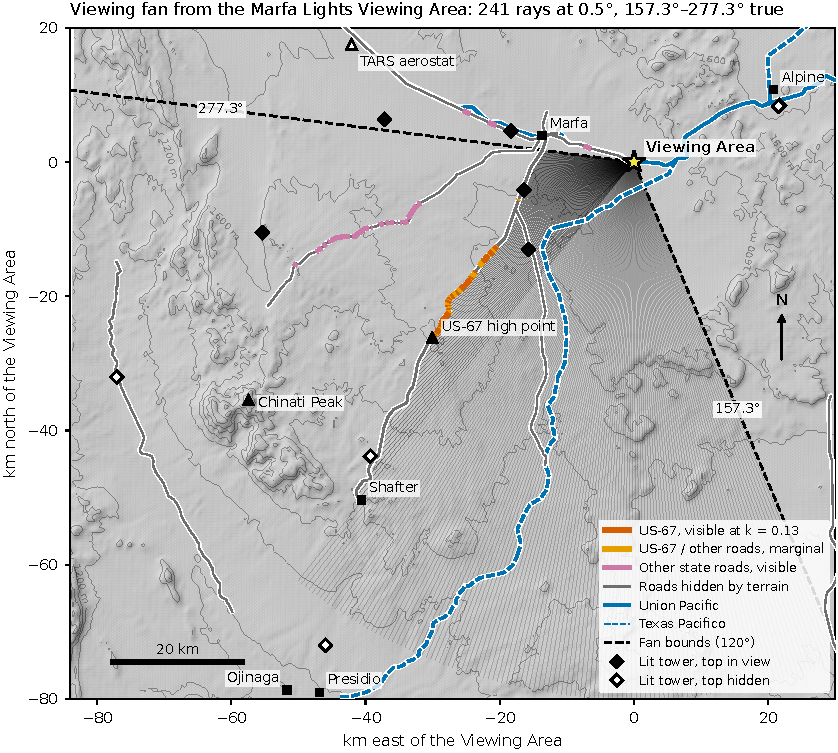
\includegraphics[width=\columnwidth]{fig01_study_area.pdf}
\caption{The view from the Marfa lights viewing area (star) toward the southwest. Roads are colored where a headlamp is in direct view of the platform (Sec.~\ref{sec:results}). Diamonds are lit communication towers. The shaded fan shows rays every $0.5^\circ$ between $157.3^\circ$ and $277.3^\circ$ true.}
\label{fig:map}
\end{figure}

\textit{Terrain.} The U.S. Geological Survey's 1-m digital elevation model from the lidar project TX\_WestTexas\_2018\_D19 (27 tiles of $10\times10$~km, collected between February and May 2019) covers every sight line of interest.\cite{USGS_lidar} Its check-point test gives a vertical root-mean-square error of 5.6~cm on open ground (565 points) and a 95th-percentile error of 21.6~cm in vegetation (461 points). Outside the lidar we use the 1/3 and 1 arc-second products. Heights are converted to ellipsoidal heights with the GEOID12B model, the one the lidar was processed with (GEOID18 differs by at most 6~cm here).\cite{NGS_geoid} From the lidar point cloud we also build a map of shrubs, fences, and buildings along the grazing corridors.

\textit{Roads and traffic.} Road centerlines come from the Texas Department of Transportation (all 821 public-road features in the area), and traffic from its annual average daily traffic (AADT) counts.\cite{TxDOT} On US-67 between Marfa and the village of Shafter the 2025 AADT is 1121 and 1383 vehicles per day at the two count stations.

\textit{Lamps, air, and eyes.} Beam patterns, signal-lamp photometry, atmospheric clarity, and the detection threshold are described in Sec.~\ref{sec:photometry}.

%=======================================================================
\section{Line of sight}\label{sec:geometry}
%=======================================================================

\subsection{An estimate}

For a smooth sphere of radius $R$, a point at distance $d$ lies below the observer's horizontal plane by $d^2/2R$. Refraction bends near-horizontal rays downward, concave toward the ground, with curvature $k/R$; the conventional ``standard'' value of the refraction coefficient is $k\approx0.13$.\cite{Hirt2010} The effective drop is therefore
\begin{equation}
\Delta h = \frac{(1-k)\,d^2}{2R}.
\label{eq:drop}
\end{equation}
At $d=30$~km this is 61~m, and the horizon of a smooth Earth for an eye 1.6~m up is only $\sqrt{2Rh/(1-k)}\approx4.8$~km away. Cars 30~km away are visible from Marfa only because the platform looks down into a basin and US-67 climbs the far side (Fig.~\ref{fig:sections}, top). Whether a given car is visible is then decided by the terrain in between, and the margins are small: the ray from a lamp at 30~km, refracted with $k=0.13$, rises only $kD^2/8R\approx2.3$~m above the straight chord at its midpoint. That is comparable to the height of a headlamp (0.66~m), much larger than the lidar error, and comparable to the 2-m error of a 30-m elevation model. This estimate sets the requirements for everything that follows.

\subsection{Exact geometry and the critical refraction coefficient}

We place the eye $O$, the lamp $T$, and terrain samples $P_i$ along the geodesic from $O$ to $T$ (computed with Karney's algorithm on the WGS84 ellipsoid\cite{Karney2013}) in Earth-centered Cartesian coordinates. For each sample we record its distance along the chord, $s_i=(\mathbf{P}_i-\mathbf{O})\cdot\hat{\mathbf u}$, and its height above the chord, $y_i=(\mathbf P_i-\mathbf O)\cdot\hat{\mathbf w}$, where $\hat{\mathbf u}$ points from $O$ to $T$ and $\hat{\mathbf w}$ is perpendicular to it in the vertical plane. Earth's curvature is then contained exactly in the $y_i$; no $d^2/2R$ approximation is needed.

With a constant refraction coefficient the ray from $O$ to $T$ is a circular arc of radius $R/k$ (Appendix~\ref{app:kcrit}), which lies above the chord by
\begin{equation}
\sigma_i(k)=\frac{k\,s_i(D-s_i)}{2R},
\label{eq:sag}
\end{equation}
where $D=|OT|$ and $R$ is the radius of curvature of the ellipsoid's normal section in the direction of the sight line (Euler's formula). The lamp is visible if the arc clears every sample, $y_i\le\sigma_i(k)$ for all $i$. Because $\sigma_i$ is linear in $k$, this is equivalent to
\begin{equation}
k\ \ge\ \kc\equiv\max_i\ \frac{2R\,y_i}{s_i(D-s_i)}.
\label{eq:kcrit}
\end{equation}
Figure~\ref{fig:geometry} illustrates this. Equation~(\ref{eq:kcrit}) turns a visibility question into a single number per lamp position: a lamp with $\kc<0$ is visible even with a straight ray, one with $\kc=0.4$ appears only in air more strongly refracting than standard, and so on. We sample the terrain every 2~m within 3~km of either end and every 5~m in between, and skip the first 5~m at the eye and the last 3~m at the lamp (the observer's own feet and the car's body). Halving the step changes no result.

\begin{figure}[t]
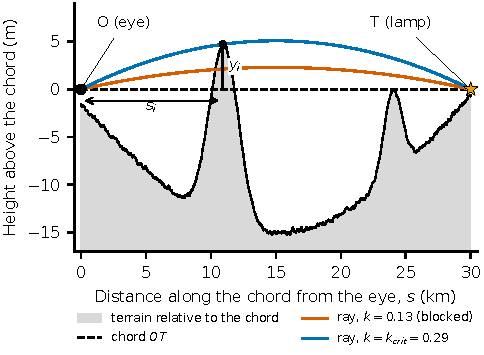
\includegraphics[width=\columnwidth]{fig00_geometry.pdf}
\caption{Line-of-sight geometry in the frame of the straight chord $OT$ (illustrative profile, 30~km). The terrain is plotted as its height $y$ above the chord, which includes Earth's curvature. A refracted ray with coefficient $k$ lies above the chord by $k s(D-s)/2R$. Here the ridge at $s_i$ blocks the standard ray ($k=0.13$); the lamp becomes visible for $k\ge\kc=0.29$.}
\label{fig:geometry}
\end{figure}

\begin{figure*}[t]
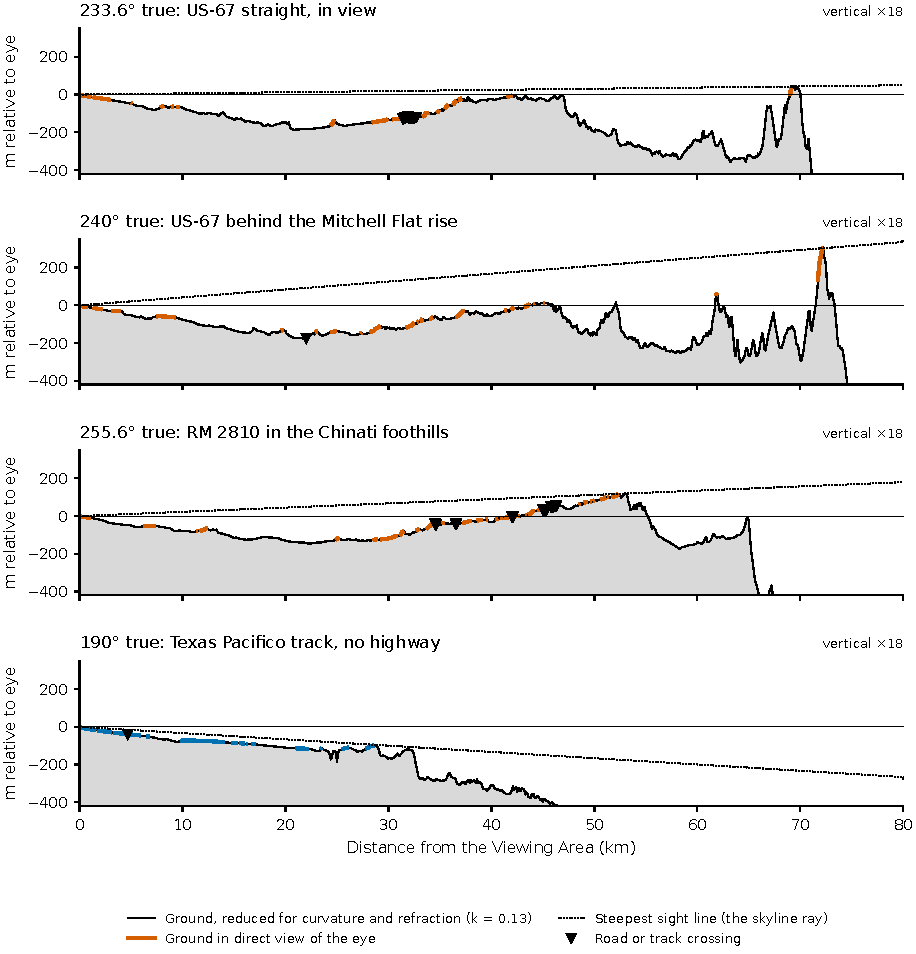
\includegraphics[width=0.72\textwidth]{fig04_sightlines.pdf}
\caption{Terrain cross-sections from the platform along four bearings, reduced for curvature and refraction ($k=0.13$) and exaggerated $18\times$ vertically. Colored: ground in direct view. Triangles: road or track crossings. Along $233.6^\circ$ the view skims the far slope that carries US-67; along $240^\circ$ a low rise hides the highway.}
\label{fig:sections}
\end{figure*}

\subsection{How robust is ``visible''?}

A visible/hidden answer from Eq.~(\ref{eq:kcrit}) is only as good as its inputs, so we attach four robustness measures to each lamp position.

\textit{Margins.} The lamp margin $d_L$ is the smallest change in lamp height that flips visibility, and $d_E$ is the same for the eye. On US-67 no visible point has a lamp margin larger than 0.84~m.

\textit{Terrain error.} We draw 200 realizations of correlated Gaussian terrain error along each sight line, with a standard deviation and correlation length for each elevation source: lidar 0.056~m (its accuracy report) with an assumed 20~m; 1/3 arc-second 0.56~m and 70~m; 1 arc-second 2.05~m and 125~m, the latter two measured against the lidar on 40\,000 points. A 0.15~m error in eye height is added. The fraction of realizations in which the lamp is visible, $P_{\mathrm{vis}}$, gives three classes: visible ($P_{\mathrm{vis}}\ge0.95$ and still visible with 0.25~m of unresolved grass added to the ground), hidden ($P_{\mathrm{vis}}\le0.05$), and marginal (the rest). In Table~\ref{tab:config}, ``robust'' uses the $P_{\mathrm{vis}}$ criterion alone. Appendix~\ref{app:mc} gives details.

\textit{Obstructions.} From the lidar point cloud (29.4 million points around the grazing corridors) we mark a 1-m cell as obstructed when it has at least two returns and at least 25\% of them more than 0.3~m above the ground, and raise it to the height of its highest return. Ground returns agree with the elevation model to a median of $-0.8$~mm.

\textit{Refraction.} Section~\ref{sec:refraction}.

%=======================================================================
\section{Refraction near the ground at night}\label{sec:refraction}
%=======================================================================

A single $k$ is a poor description of rays that graze the ground at night. For a ray at small elevation, the local coefficient follows from the vertical temperature gradient,\cite{Hirt2010}
\begin{equation}
k = 503\,\frac{P}{T^2}\left(0.0343 + \frac{dT}{dz}\right),
\label{eq:hirt}
\end{equation}
with $P$ in hPa, $T$ in K, and $dT/dz$ in K/m. At the site ($P\approx850$~hPa, $T\approx283$~K) a neutral atmosphere ($dT/dz=-0.0098$~K/m) gives $k=0.13$, an isothermal one $k=0.18$, and the gradients of 1--2~K/m that Hirt \textit{et al.}\ measured 1.8~m above grass after sunset give $k$ of 5--11.\cite{Hirt2010} We therefore also trace rays through temperature profiles that follow the terrain. In the chord frame, with elevation angles below $1^\circ$, a ray obeys
\begin{equation}
y''(s) = -\frac{k\big(a(s)\big)}{R},\qquad a = y - y_{\mathrm{ground}}(s),
\label{eq:ray}
\end{equation}
where $a$ is the ray's height above the local ground. For constant $k$ the ray through $T$ is exactly Eq.~(\ref{eq:sag}), which we use as a test. We launch a fan of rays from the eye, discard those that hit the terrain, and find the launch angles that arrive at the lamp; each is an image. The profiles are brackets, not a climatology: an exponential stable boundary layer with 3, 6, or 10~K of inversion over 50, 30, or 20~m (the standard nocturnal form\cite{Stull1988}; surface gradients 0.06, 0.2, and 0.5~K/m), an isothermal layer, a neutral one, and an elevated 4-K inversion between 40 and 60~m. They do not reach the strongest gradients measured in the lowest 2~m, which the rays at issue here cross only near the two ends.

A useful bound limits the work. If the largest local coefficient anywhere along a path is $k_{\max}$, then $y''\ge-k_{\max}/R$ with fixed end points, so every ray lies below the constant-$k_{\max}$ arc. A lamp with $\kc>k_{\max}$ is therefore hidden in that atmosphere, and need not be traced. In our profiles $k_{\max}=2.82$, which leaves 212 of the 1548 US-67 points (Marfa to Presidio, 60-m spacing) to trace.

%=======================================================================
\section{Photometry and detection}\label{sec:photometry}
%=======================================================================

\subsection{Where the platform falls in the beam}

Lamps are strongly directional, so brightness depends on where the observer sits in the lamp's own coordinates. For a car with heading $\psi$ we define the horizontal angle of the observer off the heading, positive to the driver's right, $h=\beta-\psi$ (with $\beta$ the bearing from car to observer), and the vertical angle above the lamp axis,
\begin{equation}
v = \epsilon_T - \arctan g - a,\qquad
\epsilon_T = -e_O - \frac{D}{R} + \frac{kD}{2R}.
\label{eq:angles}
\end{equation}
Here $e_O$ is the elevation of the chord at the eye, so $\epsilon_T$ is the elevation of the arriving ray above the lamp's local horizontal; $g$ is the road grade along the heading, which pitches the car; and $a$ is an aim error (zero in the central case, $\pm0.5^\circ$ in the bands). We take $g$ from the lidar $\pm25$~m along the road. On US-67 the median grade is 1.6\% and the 95th percentile 4.7\%, so pitch commonly moves the observer in the beam by $1^\circ$--$3^\circ$, as much as the geometry itself.

\subsection{Lamp intensities}

For headlamps we use the market-weighted U.S. beam patterns of the University of Michigan Transportation Research Institute: 25th, 50th, and 75th percentiles of luminous intensity on a grid from $45^\circ$ left to $45^\circ$ right and $5^\circ$ down to $7^\circ$ up, for low beams of the 20 best-selling vehicles of model year 2004 and for high beams of the same era.\cite{Schoettle2004,Schoettle2001} The median low beam has 8830~cd straight ahead, but only 55--100~cd at $30^\circ$ and a sharp upper cut-off above the horizontal; the median high beam has 37\,000~cd straight ahead. We interpolate in $\log I$. No comparable survey exists for tail and stop lamps, so we bracket them by the minimum and maximum of Federal Motor Vehicle Safety Standard No.~108: a tail lamp must give at least 2.0~cd on axis (0.8~cd at $10^\circ$, 0.3~cd at $20^\circ$) and at most 18~cd; a stop lamp 80--300~cd; the high-mounted stop lamp 25--160~cd.\cite{TP108}

\subsection{Magnitude and threshold}

At these ranges the two lamps of a car (1--1.5~m apart, $7''$--$10''$ at 30~km) are an unresolved point, and the illuminance at the eye is
\begin{equation}
E = \frac{\sum_j I_j(h,v)\,\mathcal T}{D^2},\qquad \mathcal T=\exp\!\left(-\frac{D\ln20}{V}\right),
\label{eq:illum}
\end{equation}
where $V$ is the meteorological optical range (the distance at which transmission falls to 5\%, $V=\ln 20/b$ for extinction coefficient $b$). The National Park Service reports a standard visual range at nearby Big Bend National Park of about 90~miles on average, below 55~miles on high-pollution days, and about 165~miles without pollution.\cite{NPS_BIBE} Standard visual range is defined by a 2\% contrast threshold, $3.912/b$, so $V$ is 0.766 times it: 111, 68, and 203~km, which we use as reference, least, and most favorable values. The apparent magnitude of a point source of illuminance $E$ (in lux) is\cite{Schaefer1993}
\begin{equation}
m = -13.99 - 2.5\log_{10}E.
\label{eq:mag}
\end{equation}
For example, a car 30~km away that sends 300~cd per lamp toward the platform, with $V=111$~km, gives $E=3.2\times10^{-7}$~lx and $m=+2.2$, about as bright as Polaris.

Whether the eye sees it depends on the background. Crumey's fit to laboratory contrast thresholds gives the naked-eye limiting magnitude of a point source on a background of surface brightness $\mu$ (in mag\,arcsec$^{-2}$) as\cite{Crumey2014}
\begin{equation}
m_{\mathrm{lim}} = 0.3834\,\mu - 1.4400 - 2.5\log_{10}F,
\label{eq:mlim}
\end{equation}
valid for $20<\mu<22$, where $F$ is a field factor that describes the observer and conditions (typically 1.4--2.4). The sky brightness at Marfa's horizon has not been measured, so we span $\mu=20.5$--22 and $F=1.4$--4, which gives $m_{\mathrm{lim}}=4.9$--6.6 (reference 5.9 for $\mu=21$, $F=2$).

%=======================================================================
\section{Results}\label{sec:results}
%=======================================================================

\subsection{What is in view}

Table~\ref{tab:config} gives the length of US-67 in view for a headlamp 0.66~m high at $k=0.13$, from Marfa to Presidio, for each terrain model. The three elevation models agree point by point for 98.6--99.7\% of the road, but only the lidar is accurate enough to decide visibility with confidence: with the 1-arc-second model almost all of the ``visible'' road is uncertain in the Monte Carlo, with the lidar almost all of it is robust. Measured vegetation and structures remove about 0.5~km. Of the 64.5~km between Shafter and Marfa, 9.5~km is in the visible class, 0.5~km marginal, and 54.5~km hidden. At 30-m sampling the visible road forms 29 separate stretches (five of them single samples; at the 60-m sampling used below, 18), 18--40~km from the platform, at bearings $229^\circ$--$238^\circ$ (plus one 60-m point at $251.9^\circ$), at apparent elevations between $-0.40^\circ$ and $+0.06^\circ$. Every one of them lies below the skyline, by $0.04^\circ$--$0.84^\circ$ (median $0.26^\circ$), so the lights are seen against the dark mountains rather than the sky. The limiting terrain point lies a median 3.0~km from the car.

\begin{table}[b]
\caption{Length of US-67 (Marfa to Presidio, 3095 points every 30~m) in view of the platform for a lamp 0.66~m high at $k=0.13$. ``Visible'': deterministic, $\kc\le k$; ``robust'': $P_{\mathrm{vis}}\ge0.95$; ``uncertain'': $0.05<P_{\mathrm{vis}}<0.95$.}
\label{tab:config}
\begin{ruledtabular}
\begin{tabular}{lccc}
Terrain model & Visible & Robust & Uncertain \\
 & (km) & (km) & (km)\\
\hline
1 arc-second DEM & 10.26 & 0.00 & 9.81\\
1/3 arc-second DEM & 10.26 & 0.21 & 10.71\\
1-m lidar, bare earth & 10.44 & 10.26 & 0.21\\
Lidar + obstructions & 9.93 & 9.72 & 0.27\\
\quad + 0.25 m grass & 9.36 & -- & --\\
\quad + 1 m uniform clutter & 2.04 & -- & --\\
\end{tabular}
\end{ruledtabular}
\end{table}

Other sources are few. On Ranch-to-Market Road 2810, 13~km of 52~km is in view, at $253^\circ$--$259^\circ$ and 32--53~km. The Texas Pacifico railroad is in view for 12.5~km at 3.8--8~km distance for a locomotive headlight 4~m high (9.7~km for a lamp at 1.2~m), and 10 of the 65 lit towers in the area show their top light. Lamp height matters more than refraction (Table~\ref{tab:lampk}): a truck's clearance lamps at 4~m see about 4~km more road than a car's headlamps.

\begin{table}[b]
\caption{Length of US-67 in view (km, lidar with obstructions) versus lamp height and refraction coefficient.}
\label{tab:lampk}
\begin{ruledtabular}
\begin{tabular}{lccc}
Lamp height & $k=0$ & $k=0.13$ & $k=1$\\
\hline
0.56 m (low headlamp) & 9.45 & 9.72 & 11.49\\
1.37 m (high headlamp, pickup) & 10.59 & 10.83 & 12.42\\
4.0 m (truck clearance lamp) & 13.50 & 13.77 & 15.33\\
\end{tabular}
\end{ruledtabular}
\end{table}

\subsection{Refraction}

Figure~\ref{fig:refraction}(a) shows how much road comes into view as $k$ rises: about 1.6~km more for US-67 between $k=0.13$ and 1. The main effect of refraction is on elevation, not visibility: a change $\Delta k$ lifts a light at distance $d$ by $d\,\Delta k/2R$, $0.13^\circ$ for $\Delta k=1$ at 30~km [Fig.~\ref{fig:refraction}(b)]. Table~\ref{tab:trace} summarizes the ray tracing. Even the strongest of our inversions adds only 1.5~km of visible road and lifts lights by at most $7.5'$. The elevated inversion produces three to five images of one lamp at five road points (60-m samples between 18.6 and 24.4~km from Marfa), a superior mirage, but they are only 1--8 arcseconds apart, far below the eye's resolution; they would be seen as one light, possibly twinkling. The images are stable when the step is reduced from 5 to 1~m and the fan density increased sevenfold. Surface layers whose gradient decreases monotonically with height gave single images only.

\begin{figure*}[t]
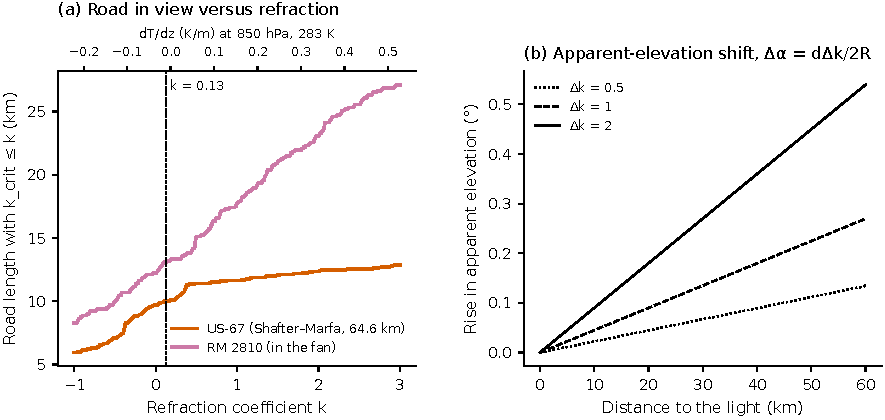
\includegraphics[width=0.8\textwidth]{fig05_refraction.pdf}
\caption{(a) Road in view (constant-$k$ model) versus refraction coefficient; the top axis gives the equivalent temperature gradient from Eq.~(\ref{eq:hirt}). (b) Rise in apparent elevation of a light for a change $\Delta k$.}
\label{fig:refraction}
\end{figure*}

\begin{table}[t]
\caption{Ray tracing through temperature profiles that follow the terrain (US-67 from Marfa to Presidio at 60-m spacing, 0.66~m lamp; the neutral case differs from Table~\ref{tab:config} through the coarser sampling). $k_{\mathrm{eq}}$: median constant $k$ that reproduces the traced arrival angle. Lift: rise in apparent elevation relative to $k=0.13$.}
\label{tab:trace}
\begin{ruledtabular}
\begin{tabular}{lccc}
Profile & Visible & $k_{\mathrm{eq}}$ & Lift, median/max\\
 & (km) & & (arcmin)\\
\hline
Neutral & 9.78 & 0.13 & 0 / 0\\
Isothermal & 9.90 & 0.18 & 0.4 / 0.6\\
Weak inversion (3 K / 50 m) & 10.86 & 0.30 & 1.4 / 1.7\\
Moderate (6 K / 30 m) & 10.92 & 0.47 & 2.9 / 4.3\\
Strong (10 K / 20 m) & 11.28 & 0.67 & 4.5 / 7.5\\
Elevated, 40--60 m & 9.66 & 0.36 & 1.8 / 2.8\\
\end{tabular}
\end{ruledtabular}
\end{table}

\subsection{Brightness}

US-67 runs almost straight at the platform. A northbound car (toward Marfa) has the platform $3^\circ$--$33^\circ$ to the driver's right (5th--95th percentile; median $14^\circ$), and $0.6^\circ$ below to $2.5^\circ$ above the lamp axis, near the top of the low beam [Fig.~\ref{fig:headlights}(a,b)]. Table~\ref{tab:phot} and Fig.~\ref{fig:headlights}(c) give the result. A northbound car is a naked-eye light over at least 87\% of the road in view for every lamp percentile, visual range, and threshold we tried, and over 93\% at the reference values: typically magnitude $+2.6$ on low beam and $+0.4$ on high beam. On the straight at $233.7^\circ$ (31--33~km) it reaches $-1.7$ on low beam and $-2.4$ on high beam, brighter than Sirius ($-1.46$). A southbound car shows its tail lamps $3^\circ$--$33^\circ$ off its rear axis (5th--95th percentile). At the regulatory minimum they are invisible ($m\approx9$); at the maximum they are at the threshold ($m\approx5.6$); braking brings them to $m\approx4.6$ even at the minimum, visible over most of the road. A red light on these bearings is therefore most likely a braking car.

\begin{figure*}[t]
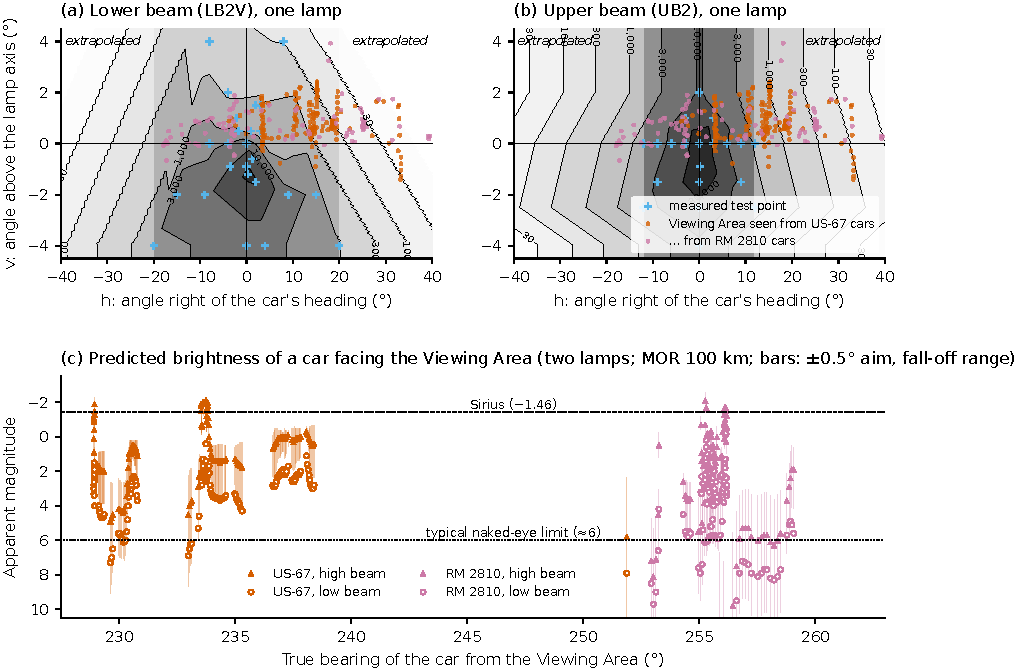
\includegraphics[width=0.92\textwidth]{fig03_headlights.pdf}
\caption{(a,b) Median U.S. low- and high-beam patterns (one lamp, candela), with the platform's position in the beam of northbound cars on US-67 (orange) and of cars on RM~2810 facing the platform (pink). (c) Predicted magnitude of one car on the stretches of US-67 in view ($V=111$~km, $k=0.13$): northbound headlamps (circles: low beam, bars 25th--75th percentile of the fleet; triangles: high beam) and southbound tail lamps (filled squares: regulatory maximum; open: minimum; crosses: braking at the minimum). Band: naked-eye limit, Eq.~(\ref{eq:mlim}).}
\label{fig:headlights}
\end{figure*}

\begin{table}[t]
\caption{Predicted magnitude of one car on US-67 (Shafter--Marfa) where its lamps are in view, and the road length over which it is brighter than $m_{\mathrm{lim}}$: reference ($V=111$~km, $\mu=21$, $F=2$, $m_{\mathrm{lim}}=5.9$) and full bracket (least favorable $V=68$~km, $\mu=20.5$, $F=4$; most favorable $V=203$~km, $\mu=22$, $F=1.4$). Road sampled every 60~m; ``in view'' means $P_{\mathrm{vis}}\ge0.5$ for the lamp's height.}
\label{tab:phot}
\begin{ruledtabular}
\begin{tabular}{lccc}
Lamps & $m$, median & Detectable & Bracket\\
 & (range) & (km) & (km)\\
\hline
\multicolumn{4}{l}{\textit{Northbound, 10.0 km in view}}\\
Low beam, 25th pct. lamp & 2.9 ($-1.4$ to 6.8) & 9.4 & 8.7--10.0\\
Low beam, fleet median & 2.6 ($-1.7$ to 6.0) & 9.6 & 9.0--10.0\\
High beam, fleet median & 0.4 ($-2.4$ to 5.4) & 10.0 & 9.3--10.0\\
\multicolumn{4}{l}{\textit{Southbound, 10.1 km in view}}\\
Tail lamps, FMVSS min. & 9.1 (7.9 to 10.6) & 0 & 0\\
Tail lamps, FMVSS max. & 5.6 (4.7 to 6.3) & 6.7 & 0--10.1\\
Braking, FMVSS min. & 4.6 (3.7 to 6.1) & 9.4 & 4.4--10.1\\
\end{tabular}
\end{ruledtabular}
\end{table}

\subsection{One car in time}

Figure~\ref{fig:onecar} follows a northbound car at 30~m/s. It takes 13.6 minutes to cross the region in view and is visible for 334~s of it, in 18 separate windows: a median 510~m of road (17~s), from 60~m (2~s, our sampling limit) to 2.1~km (70~s). While visible it drifts across the view at about $0.9^\circ$ per minute, never more than $0.84^\circ$ below the skyline. Within a window its brightness changes by a median of 1.1 magnitudes (up to 4.9), and between successive 2-s samples by up to 0.8 magnitudes in one case in ten, with no change in the car: grade changes pitch the beam by degrees across the top of the low beam, where intensity falls by a factor of about 2 per degree, and curves swing the heading.

One ordinary car therefore produces a light that appears, drifts, brightens and dims, vanishes, and reappears a little further on, 18 times. (The 18 windows are the 29 stretches of Sec.~\ref{sec:results}A at coarser sampling.) For a one-way flow $q$ with random arrivals, the number of cars in view is Poisson distributed with mean
\begin{equation}
N = \frac{qL}{u},
\label{eq:occupancy}
\end{equation}
where $L$ is the length of road in view and $u$ the speed. With $L=10.0$~km and $u=30$~m/s, $N=0.93$ per 10 vehicles per hour in each direction. At the daily-mean flow implied by the AADT (23--29 vehicles per hour each way), two or three northbound headlights would be in view at any moment; at night the flow is lower by a factor we have not measured.

\begin{figure*}[t]
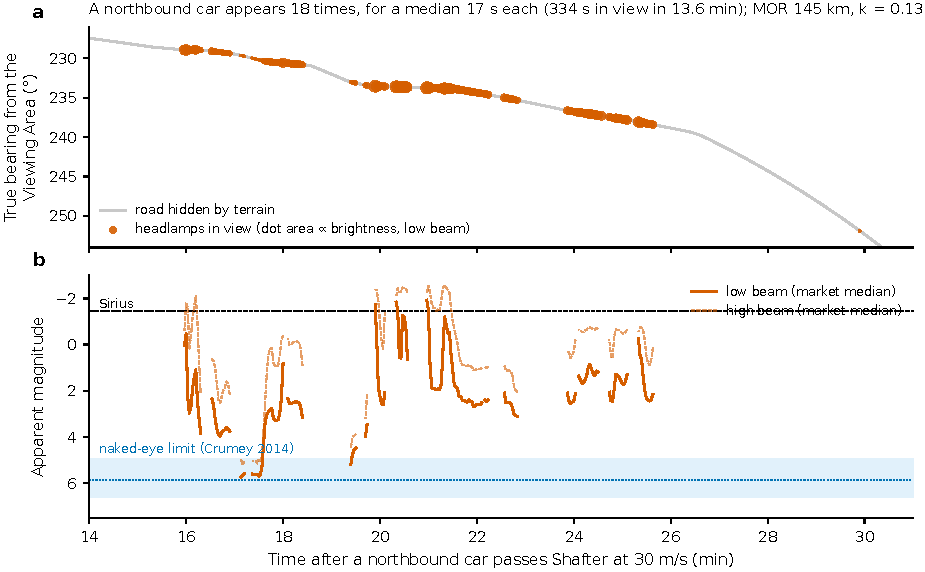
\includegraphics[width=0.8\textwidth]{fig08_one_car.pdf}
\caption{A northbound car on US-67 at 30~m/s, seen from the platform. (a) Bearing versus time; orange where the headlamps are in view (dot area increases with brightness), grey where terrain hides the road. (b) Magnitude on low beam (solid) and high beam (dashed), fleet median, $V=111$~km.}
\label{fig:onecar}
\end{figure*}

\subsection{A check against photographs}

The geometry can be checked against photographs taken from the platform. On 21 November 2018, 20--35 minutes after sunset, the author photographed the US-67 sector with a 210-mm lens on an APS-C camera (nominally 936 pixels per degree).\footnote{The camera's clock was found to be 59~min fast by matching a sunset frame to the Sun's computed position.} We registered each frame by fitting a four-parameter camera model (azimuth, elevation, roll, scale) to the modeled skyline, with residuals of 0.005--0.017$^\circ$, and then located point lights in the short exposures with a detection that does not use the road model [Fig.~\ref{fig:photos}(a)]. Grouping detections in frames seconds apart gives eight independent sightings. Their median angular distance from the modeled visible road is $0.0085^\circ$ (8 pixels, about 4~m at 26~km), whereas random positions in the same band of the frames have a median distance of $0.28^\circ$; the probability that at least half of eight random positions fall that close is $3\times10^{-6}$ [Fig.~\ref{fig:photos}(c)]. About half of the road that falls in these frames is modeled as hidden, yet all eight sightings lie on visible stretches; if the visible/hidden split had no predictive power, the chance of this would be the product of each frame's visible fraction, about 0.005. One light seen in two frames 6~s apart moved $179\pm30$~m along the road, 30~m/s (17--48~m/s at $2\sigma$). A 45-s exposure records the traffic as a streak that follows the modeled road [Fig.~\ref{fig:photos}(b)].

This is a test of internal consistency, not of absolute pointing: because the frames are registered to the modeled skyline, an error common to skyline and road would not show. It also does not test brightness (the frames are not photometrically calibrated) or refraction (the elevation zero point is degenerate with $k$).

\begin{figure*}[t]
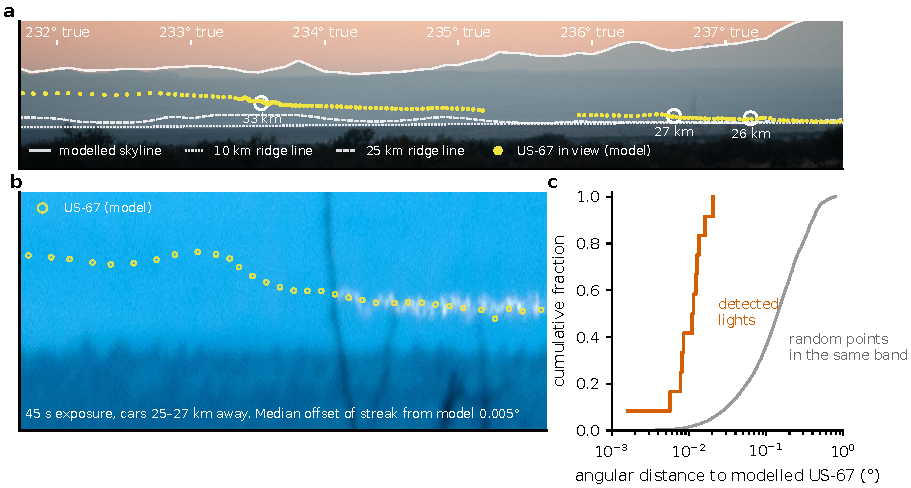
\includegraphics[width=0.92\textwidth]{fig07_photo_validation.pdf}
\caption{Check of the geometry against photographs from the platform, 21 November 2018. (a) Detected lights (circles, with distances) and the modeled US-67 in view (dots), with the modeled skyline and ridge lines. (b) A 45-s exposure; the streak, found without reference to the model, lies a median $0.005^\circ$ from the modeled road (circles). (c) Cumulative distribution of the distance from detected lights to the modeled road, and of random positions in the same band.}
\label{fig:photos}
\end{figure*}

%=======================================================================
\section{Discussion}\label{sec:discussion}
%=======================================================================

\textit{What the model explains.} Several features of reported sightings follow from ordinary physics. The lights sit just below the skyline because the only road in view lies on the far slope of the basin, seen against the mountains within $0.84^\circ$ of their crest. They appear and vanish without moving much because terrain cuts the road into short windows. They can be startlingly bright, brighter than any star, where the road points at the platform and the car pitches its beam upward. They brighten and fade within a single appearance because grade and curvature move the observer across the low-beam pattern. They seem too far away to be cars because the eye has no distance cue for a point source, and a light 30~km off at magnitude $+2$ looks like a star. Refraction adds only minutes of arc of lift and, in our profiles, no resolvable splitting.

\textit{What it does not show.} A model of where ordinary lamps can appear does not prove that any particular sighting was a car. It also does not cover every source: private ranch roads, ranch lights, off-road vehicles, and aircraft are not catalogued. Conversely, it defines where a light would be hard to explain. Combining the sources above with traffic rates, we find that in the band within 5~mrad below the skyline, about 80\% of the view has an expected rate of catalogued transient lights below 0.01 per hour and no fixed light. This estimate assumes that 2\% of the daily traffic passes in a night hour, that a quarter of drivers use high beams, and that a light's position is known to $\pm0.3^\circ$ in azimuth and $\pm0.1^\circ$ in elevation; with coarser positions the quiet fraction shrinks quickly. A light that appears there, or that stays steady for minutes, or that moves against the direction of the road, would not be explained by this model, and would deserve careful measurement.

\textit{Limitations.} The largest are in the photometry. The beam survey describes lamps of about 2004; modern LED headlamps have sharper cut-offs and different wide-angle light, which the fleet percentiles do not cover. Signal lamps are bracketed by regulation, not measured. Pitch is approximated by the road grade, and the horizon sky brightness and the observer's field factor are not known for this site. The headlamp conclusion is insensitive to these; the tail-lamp result is not. In the geometry, grass lower than about 0.3~m is below what the lidar resolves (allowing for 0.25~m of it removes 0.6~km of visible road), and the refraction profiles are brackets, not measurements.

\textit{For students.} Each piece of the model can be done by hand or in a short program: the curvature drop and horizon distance [Eq.~(\ref{eq:drop})]; the critical coefficient for a single ridge [Eq.~(\ref{eq:kcrit})]; the magnitude of a car of known intensity [Eqs.~(\ref{eq:illum}) and (\ref{eq:mag})]; the occupancy of a road window [Eq.~(\ref{eq:occupancy})]. A class with access to a dark roadside viewpoint can repeat the whole analysis for a local ``ghost light'' with free national elevation data.

%=======================================================================
\section{Conclusions}
%=======================================================================

Exact geometry on 1-m lidar terrain shows that about 10~km of US-67, in 29 short stretches 18--40~km away, is in view of the Marfa lights viewing area, always just below the skyline. A single number, the critical refraction coefficient, decides visibility for each lamp position; because rays graze the ground within a meter or two, only lidar terrain with a terrain-error Monte Carlo makes that decision robust, and nocturnal inversions of up to 0.5~K/m at the surface change it little. Market-weighted beam patterns and a contrast-threshold model show that a northbound car there is a naked-eye light over nearly all of the road in view, typically of second or third magnitude and sometimes brighter than Sirius, while tail lamps are near the limit of vision. A single car should appear some 18 times in a quarter of an hour, brightening and fading with the road's grade and curves. The model makes these ordinary lights predictable in position, brightness, and timing, and so marks the rest of the view as the place to look for anything else.

\begin{acknowledgments}
[To be added at conditional acceptance.]
\end{acknowledgments}

\section*{Author declarations}
\textit{Conflict of interest.} The author has no conflicts to disclose.

\textit{Data availability.} All code, derived data, figures, and a manifest (URLs and SHA-256 checksums) of the public source data are available at \repo. The photographs are available from the author on request.

\textit{Use of AI tools.} [Author to review before submission.] In accordance with AIP Publishing's policy, we disclose that an AI system (Claude, Anthropic; configured model identifier claude-opus-5-5, 2026) was used to write and test the analysis code, to extract tabulated values from source documents (the UMTRI and FMVSS photometric tables, checked cell by cell against the printed tables), and to draft text. It was used because the project was carried out by a single author. All code is public and covered by unit tests, and every number in this paper is produced by that code.

\appendix

\section{The refracted ray and the critical coefficient}\label{app:kcrit}

In a horizontally stratified atmosphere with refractive index $n(z)$, a ray at elevation angle $e$ bends toward the denser air with curvature $\kappa=-(1/n)(dn/dz)\cos e$. Writing $\kappa=k/R$ defines the refraction coefficient; with $n-1\propto P/T$ and hydrostatic pressure this gives Eq.~(\ref{eq:hirt}). In the chord frame and for small angles, $y''=-k/R$. With constant $k$ and $y(0)=0$, the ray is $y=\theta s-ks^2/2R$; requiring $y(D)=0$ gives $\theta=kD/2R$ and $y=ks(D-s)/2R$, Eq.~(\ref{eq:sag}). The relative error of the parabolic approximation is of order $(D/R)^2\approx10^{-5}$. The apparent elevation of the lamp is the chord elevation plus $\theta$, and a change $\Delta k$ raises it by $D\Delta k/2R$.

\section{Terrain-error Monte Carlo}\label{app:mc}

Each elevation source (lidar, 1/3 and 1 arc-second) gets its own, independent error field along the sight line. For a source with correlation length $\ell$ we generate a unit-variance first-order autoregressive sequence on a uniform grid of spacing $g=\min(\ell/4,\,5~\mathrm{m})$, $\delta_{j+1}=\phi\,\delta_j+\sqrt{1-\phi^2}\,\xi_j$ with $\phi=e^{-g/\ell}$ and independent standard normal $\xi_j$; this has the exponential correlation $e^{-|\Delta s|/\ell}$. We interpolate it linearly to the terrain samples, restore unit variance (interpolation lowers it by at most 6\%), and multiply by the standard deviation $\sigma$ of the source that supplied each sample. The values for the 1/3 and 1 arc-second models were measured against the lidar on about 40\,000 points; the lidar $\sigma$ comes from its accuracy report and its 20~m correlation length is assumed. An independent eye-height error ($\sigma=0.15$~m) tilts the chord, adding $\delta_{\mathrm{eye}}(D-s)/D$. For each of 200 realizations the lamp is visible if the perturbed terrain stays below the ray; $P_{\mathrm{vis}}$ is the fraction of realizations in which it does. Only samples that could reach the ray within $6\sigma$ are evaluated. Unit tests confirm the error statistics, the deterministic limit, and the analytic probability for a pure eye-height error.

\section{Verification}\label{app:verify}

Thirty unit tests cover the geometry (Euler radius, smooth-Earth horizon distances for $k=0$, 0.13, 0.5; $\kc$ against brute force on random terrain; an isolated ridge; margins flipping visibility), the Monte Carlo, the ray tracer (constant-$k$ reproduction; the reach of a surface duct against its analytic value), and the photometry (tabulated beam values; the magnitude scale; the definition of visual range; the sign conventions of $h$ and $v$). Run with the settings of an earlier, independent implementation (1-arc-second terrain, 15-m step), the model agrees on visibility for 1075 of 1077 points; the earlier implementation's azimuths were $0.12^\circ$ too large, from mixing spherical and ellipsoidal geometry. Changing the terrain step from 2/5~m to 1/2~m changes none of 3095 results.

\bibliography{refs}

\end{document}
